\section{External Renderer}
\label{chapter:design:renderer}

	Luckily, the usage of an external renderer already provides access to an advanced API. Users knowledgeable about the external graphics engine being used can fine-tune operations within that engine. Any object controlling the rendering process is created within the PURGE namespace, and adopted by the external rendering facility, the \classname{Renderer}. That facility is responsible for taking that object into account during the rendering process.

	\begin{figure}[htbp]
		\centering
		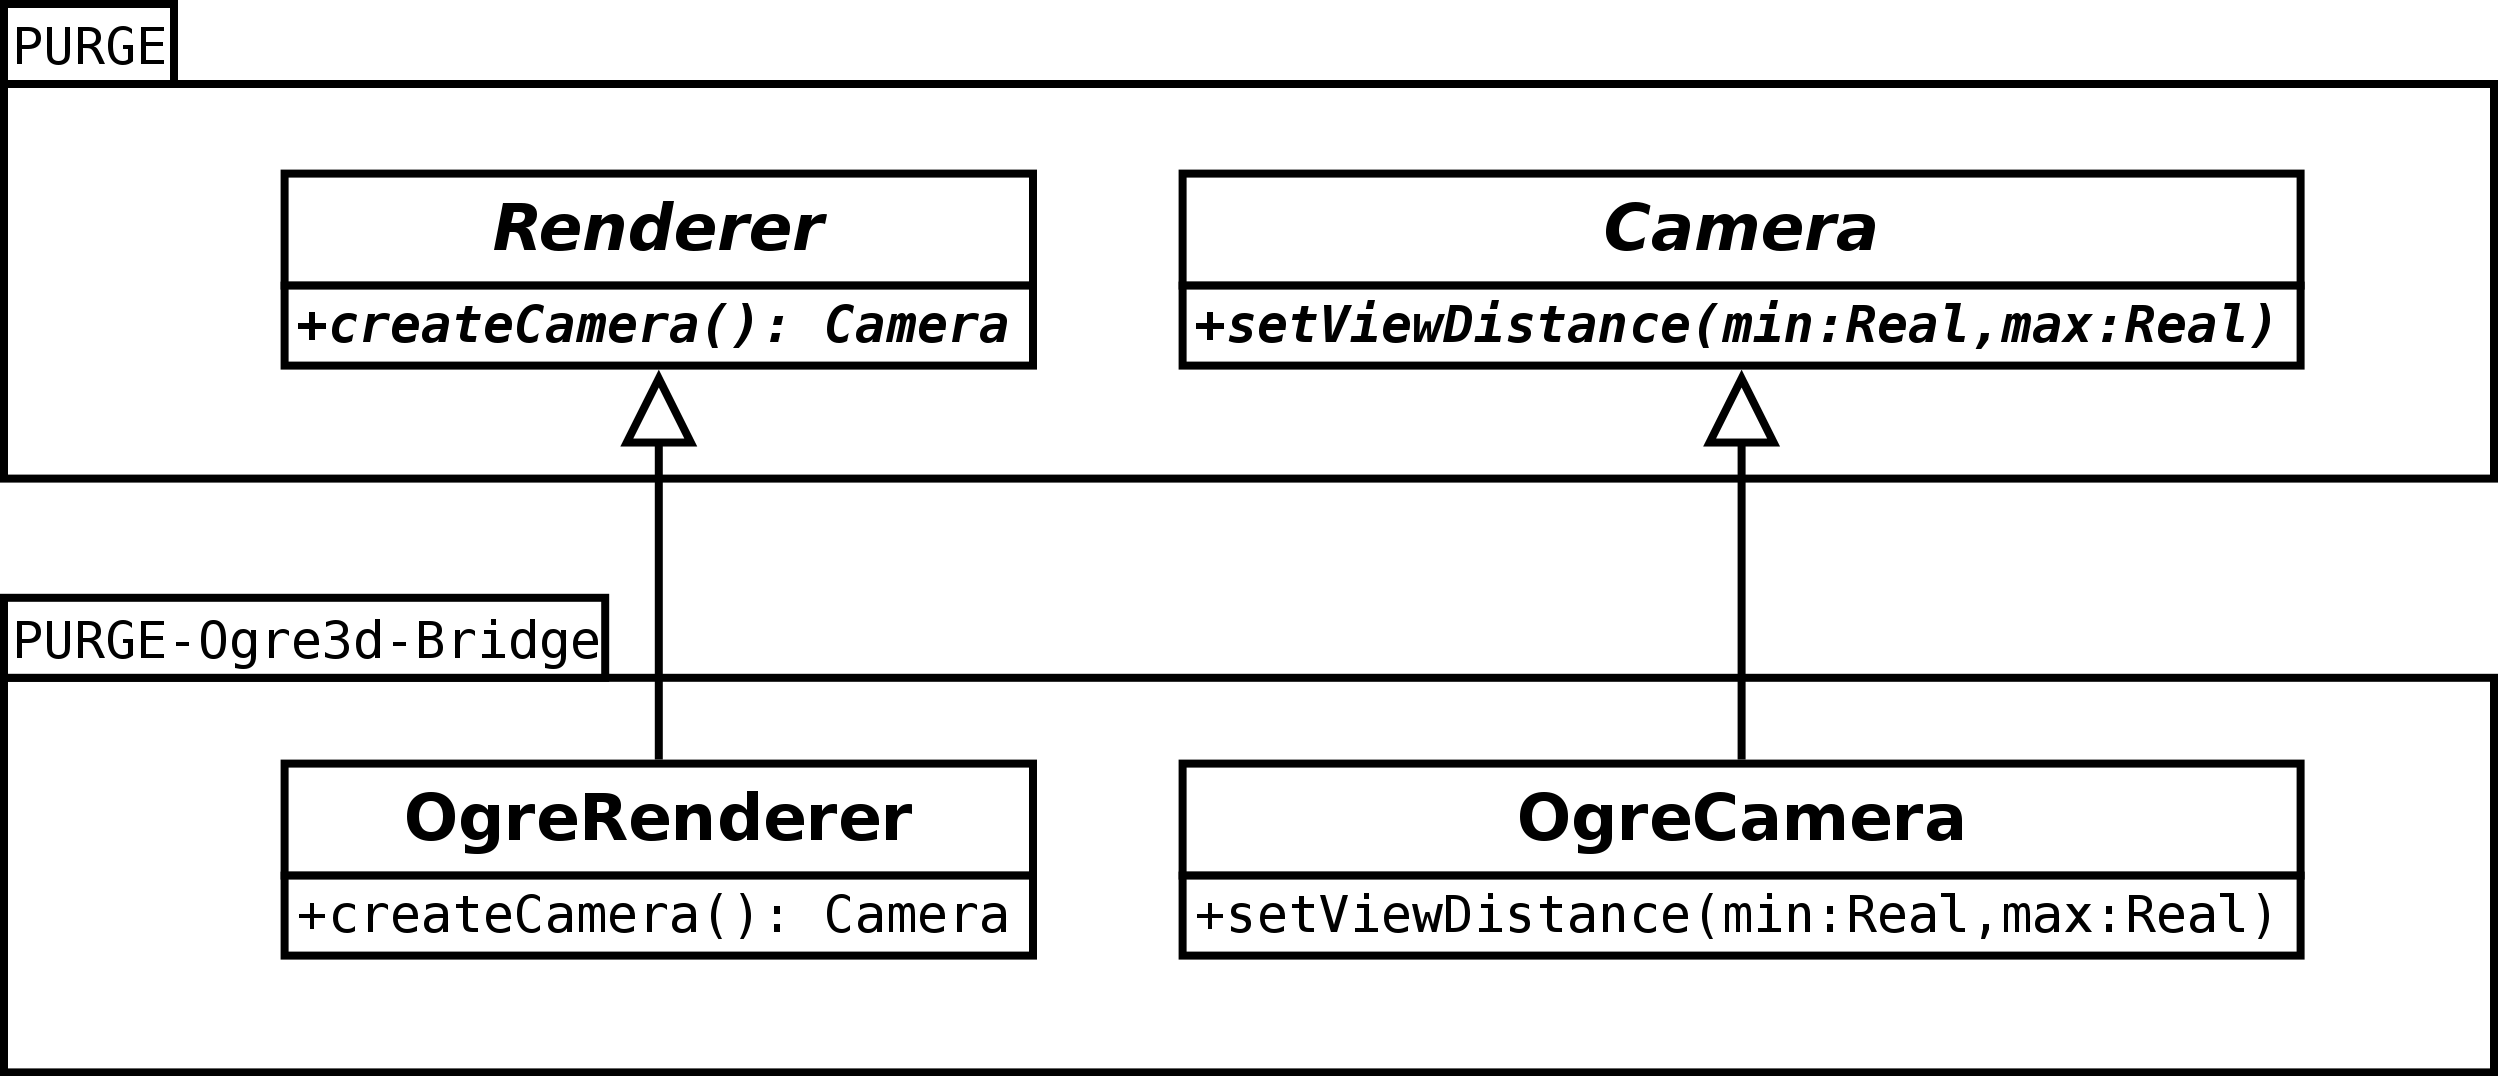
\includegraphics[width=14cm]{images/RendererArchitecture1.png}
		\caption{Initial design approach to the external renderer}
		\label{fig:RendererArchitecture1}
	\end{figure}

	The first approach to the integration of the external render was to design the \classname{Renderer} as an abstract class that is responsible for providing all other objects supported by PURGE, as seen in Figure \ref{fig:RendererArchitecture1}. The drawback of this architecture became clear quite early during the implementation process: The design of PURGE was adopting too many characteristics of the underlying renderer. The library was becoming a layer on top of Ogre3d instead of an independent graphics library.

	To counter this trend during the design process, the architecture was slightly altered to decouple PURGE objects from their implementations in the renderer. The aim was to render the \classname{Renderer} completely interchangeable, even at run-time, an approach to the engine design we have found in \cite{Plummer2004}\footnote{Plummer basically contemplates on a game architecture proposal in \cite{Rollings:2003:GAD:1209229} and attempts to create a game engine with completely interchangeable components for specialized tasks.}. This has lead to the second design outlined in Figure \ref{fig:RendererArchitecture2}, where the objects in PURGE can survive an exchange of the active \classname{Renderer}. We switched from direct inheritance to the bridge pattern as described in \cite{GOF}.

	\begin{figure}[htbp]
		\centering
		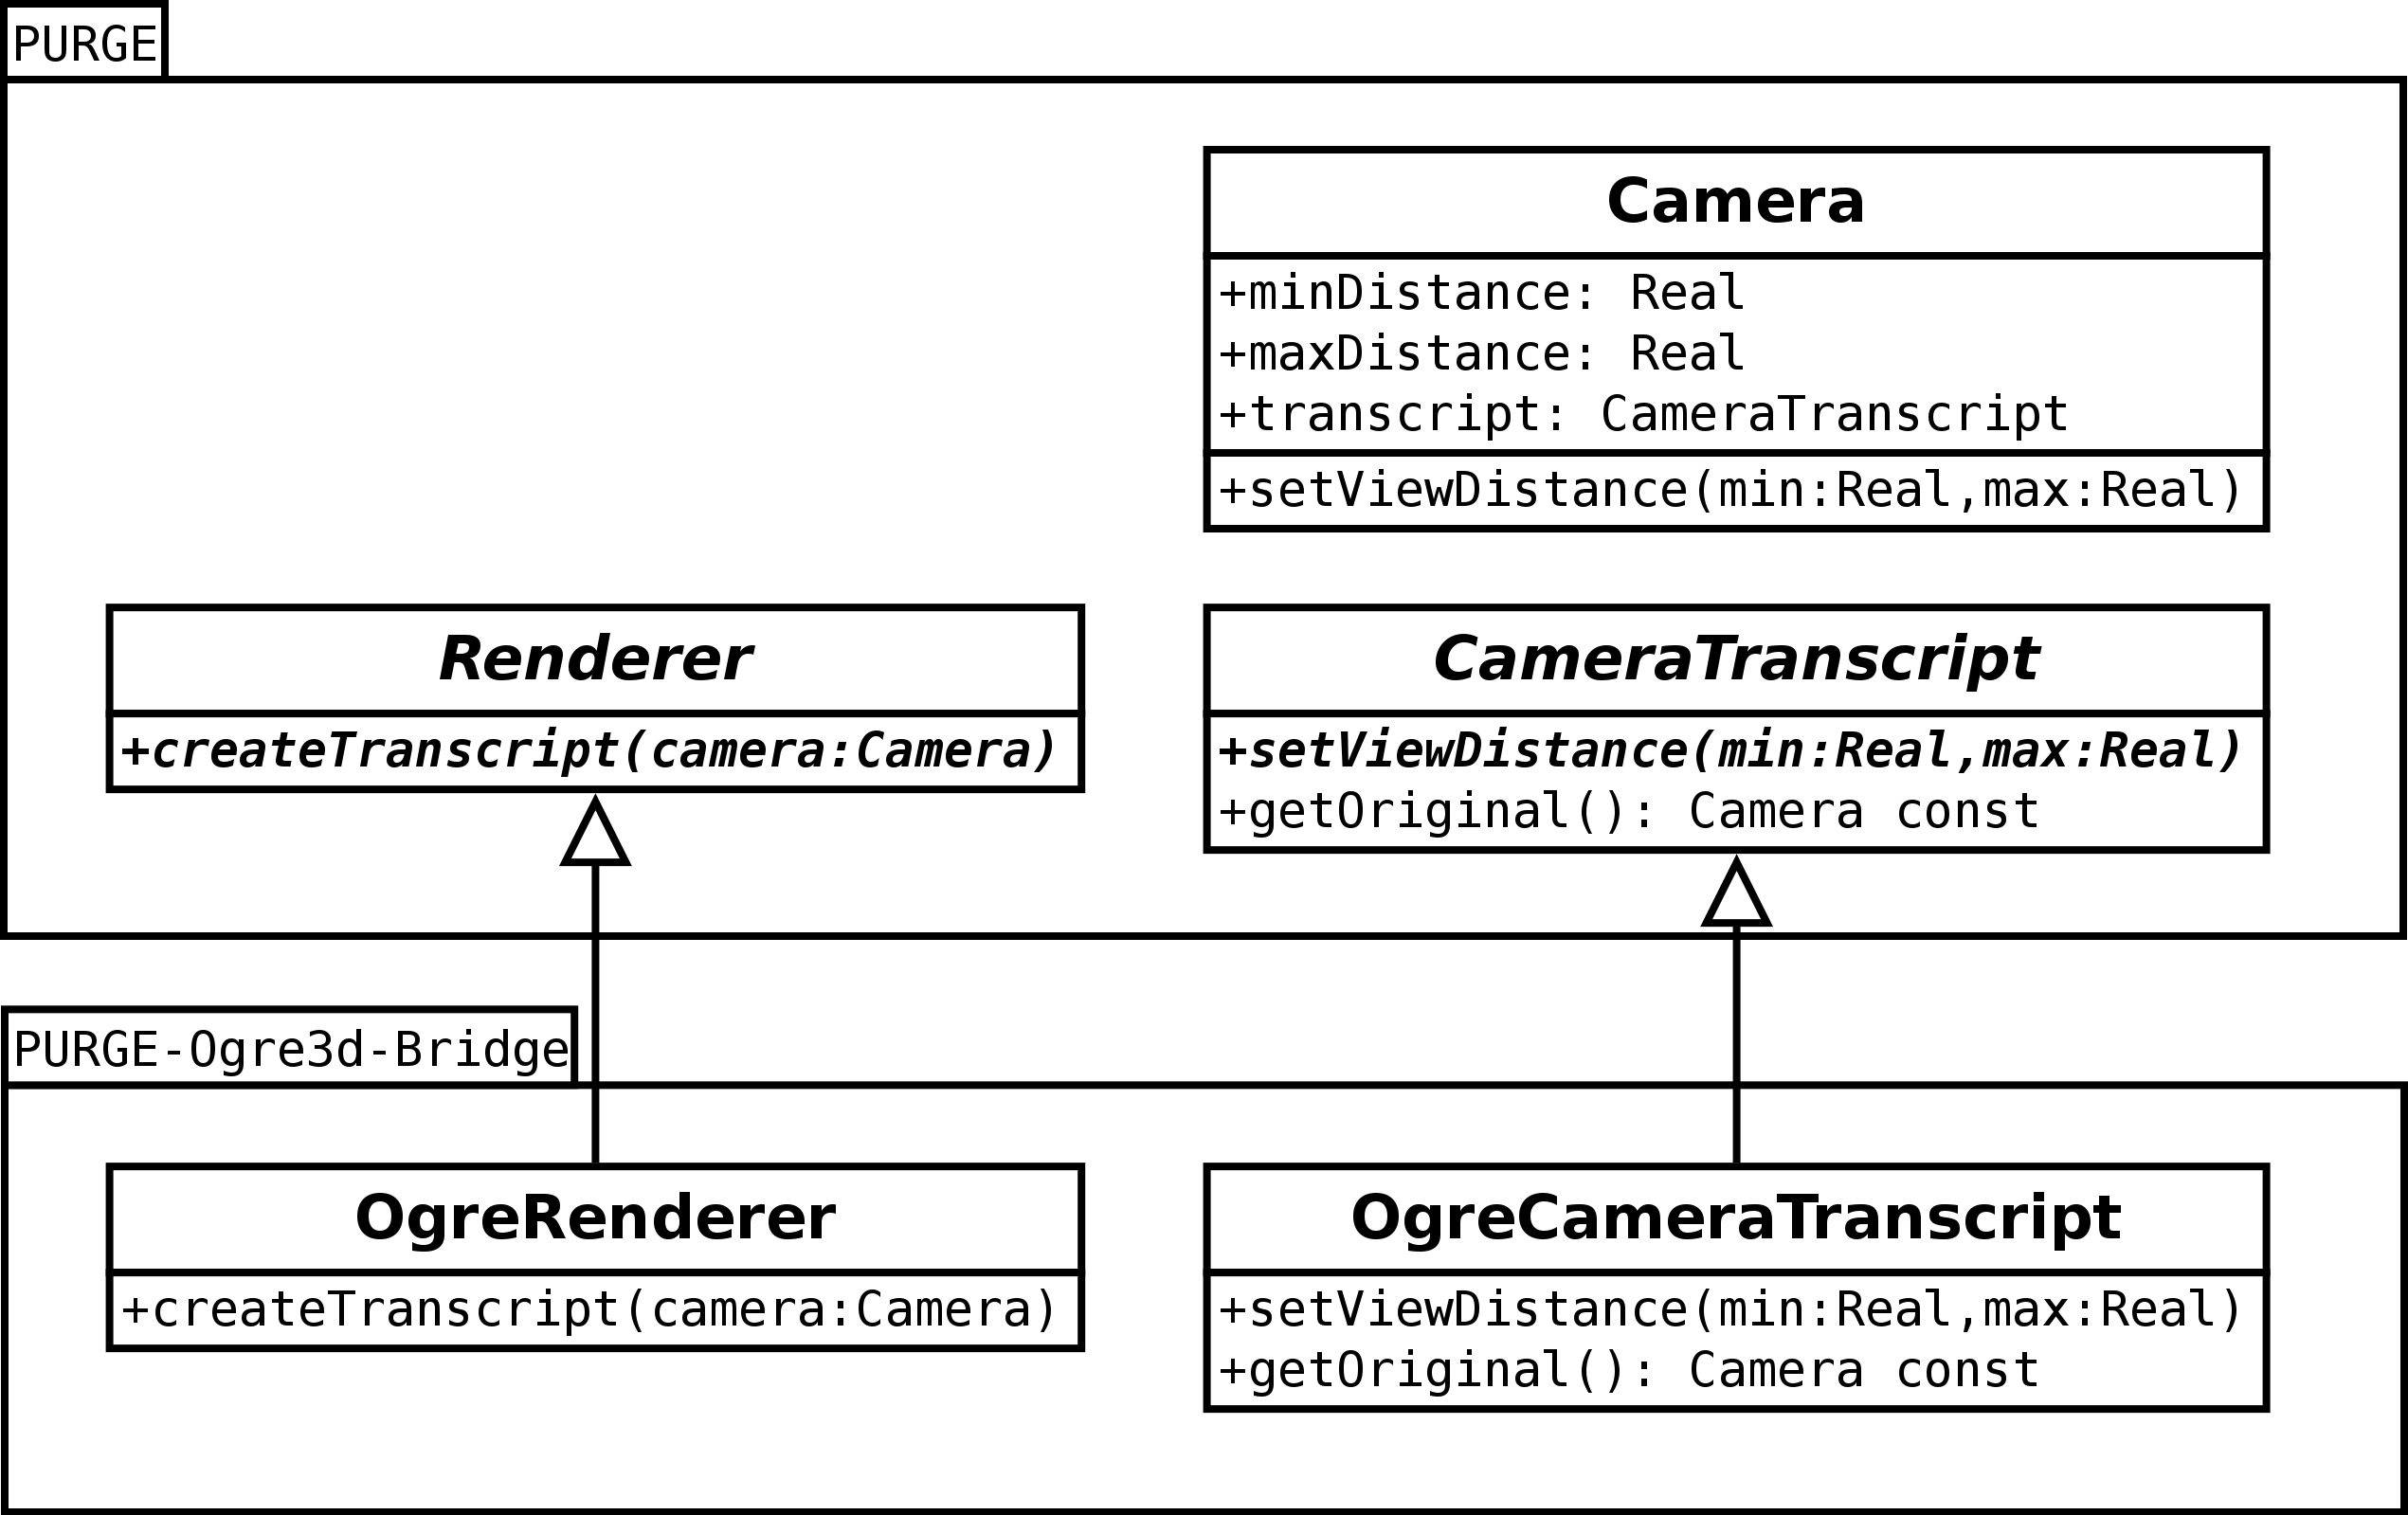
\includegraphics[width=14cm]{images/RendererArchitecture2.png}
		\caption{Second design of the external renderer}
		\label{fig:RendererArchitecture2}
	\end{figure}

	But this change had some drawbacks: Although the PURGE object was now capable of storing its parameters, the API had not changed. The object would now store its state on its own, but immediately update the implementing object. Apart from this lack of solution to the initial problem, another, more grave design flaw was brought to our attention with this switch. Why should the library actually enforce the duplication of the already-present data in the \classname{Renderer}?
			
	What was the \classname{Transcript} good for? It was a required implementation detail in the initial design, but the usage of the bridge pattern had made that class obsolete for PURGE. The \classname{Renderer} was still free to create a mapping of a PURGE-object to its own, graphics-engine specific objects, but PURGE does not need any information from these objects.
	
	So this short-lived solution was discarded and the flow of information was reversed: Instead of pushing any changes from PURGE to the \classname{Renderer}, the \classname{Renderer} is now expected to pull any information it needs from PURGE. The outline of this design can be seen in Figure \ref{fig:RendererArchitecture3}.

	\begin{figure}[htbp]
		\centering
		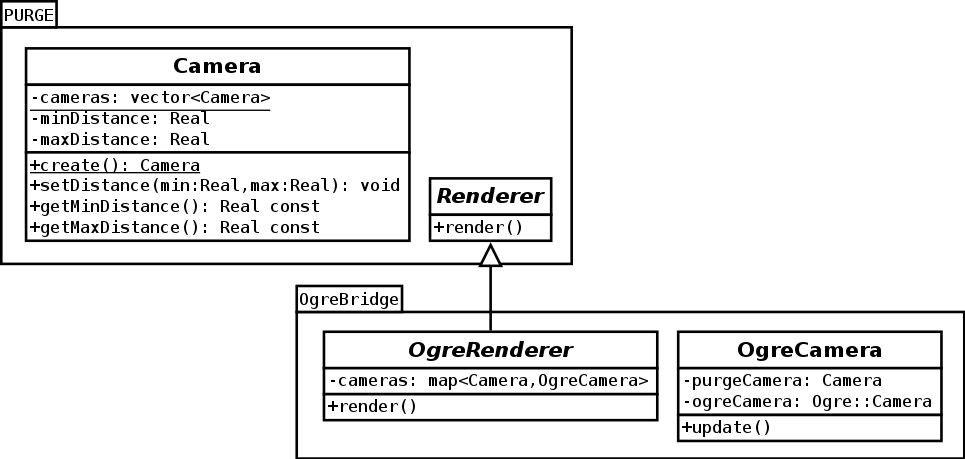
\includegraphics[width=14cm]{images/RendererArchitecture3.png}
		\caption{Third iteration of the renderer architecture}
		\label{fig:RendererArchitecture3}
	\end{figure}

	With this last change, the flow of information is defined as follows:
	
	\begin{numlist}
		\item The application can create, update and delete any number of objects in PURGE. None of the changes have any visible effect at this point.
		\item When all changes for this loop cycle are declared to PURGE, the rendering step initiates.
		\item The \classname{OgreRenderer} is responsible for creating, updating and deleting all required internal objects to render the scene as contained in PURGE.
		\item When the renderer is finished, control is passed back to PURGE, where a new loop cycle begins.
	\end{numlist}

	The implementation of this communication model requires further elaboration on the details of the render loop. We will come back to the implementation specifics in Section \ref{chapter:implementation:renderer}.

